% ------ headers globales y begin ---------------
\documentclass[11pt, a4paper, twoside]{article}
\usepackage{header_tp2}

\begin{document}{}
% -----------------------------------------------

\begin{paragraph}\

Para demostrar la correctitud dividiremos el proceso en dos subprocesos
independientes. Por un lado, demostraremos que el algoritmo expuesto cumple
con los parámetros de un ``Algoritmo de Kruskal''. Por otro lado,
demostraremos que un ``Algoritmo de Kruskal'', mediante su invariante de
ciclo, cumple con las condiciones de nuestro problema.

\end{paragraph}

\begin{paragraph}\

\centerbf{Veamos que cumple Kruskal}

Veamos que nuestra implementación es una correcta versión del algoritmo de
Kruskal. En cada iteración, Kruskal agrega a sus aristas la arista con menor
peso entre las que no forman ciclo con las que ya tiene. Es decir, que una dos
nodos que no estaban conectados por ningún camino, o lo que es lo mismo, que
pertenezcan a distintas componentes conexas.

Veamos que nuestro algoritmo elige la misma arista que Kruskal. Iteramos sobre
todas las componentes y elegimos las dos que tienen la menor distancia hacia
otra componente. Ahora veamos que las distancias de una componente hacia otra
están bien calculadas.

En la etapa de inicialización, cuando tenemos n componentes conexas triviales,
la distancia entre cualquier par de ellas es la distancia euclidea entre sus
únicos nodos. Ahora la distancia entre dos componentes conexas no triviales,
es, afín a la noción de distancia en conjuntos, la distancia más corta entre
un nodo de una componente conexa y un nodo de la otra. Supongamos que
conocemos la distancia de la componte conexa A hacia la B y la C. Luego la
distancia entre A y $B \cup C$ es la distancia entre un nodo de A y un nodo de
B o C, es decir el mínimo de la distancia mínima entre un nodo de A y un nodo
de B, y la distancia mínima entre un nodo de B y un nodo de C. Se concluye
esta relación: distancia entre A y $B \cup C$ = min(distancia entre A y B,
distancia entre A y C).

\end{paragraph}

\begin{paragraph}\

\centerbf{Veamos que Kruskal soluciona nuestro problema}

\begin{aclaracion}

Se cometerá un abuso de notación al indicar que se \emph{``suma/resta una
arista a una solución''}; lo que se está realizando es realmente agregar o
quitar la arista del conjunto de aristas de la solución. Se denotará $S_{n}$
como \emph{``el grafo solución de n componentes conexas''}.

\end{aclaracion}

Queremos demostrar que, partiendo de un grafo inicial $S_{n}$, compuesto por
$n$ componentes triviales, el resultante de aplicar $k$ iteraciones de
Kruskal, $S_{n-k}$, es una solución óptima. Para ello, aplicaremos inducción.

\end{paragraph}

\begin{paragraph}\
%
%- Hipótesis Inductiva
%
\begin{center}
\textbf{PREMISA INDUCTIVA}\\
<<\texttt{P(i)}>>
\end{center}

La solución $S_{n-i}=(V,E_{n-i})$, subgrafo generador de $K_n$, obtenida luego
de aplicar $i$ veces Kruskal, la cual tiene <<$n-i$>> componentes conexas,
minimiza la \textbf{función objetivo} $f$ (\ref{ej2-funcionobjetivo}, pág.
\pageref{ej2-funcionobjetivo}) cuando se la contrasta contra cualquier otra
solución compuesta por <<$n-i$>> o menos componentes conexas.

\end{paragraph}

\begin{paragraph}\
%
%- Caso Base
%
\begin{center}
\textbf{CASO BASE}\\
<<\texttt{P(1)}>>
\end{center}

Resulta trivial, ya que cualquier grafo de $n$ nodos que contiene <<$n-1$>>
componentes conexas contiene a lo sumo una sola arista, ya que por absurdo:
dado cualquier grafo que cumpla las condiciones anteriores, al intentar
agregar una segunda arista resulta inevitable unir dos de las <<$n-1$>>
componentes conexas restantes, ya que todas son trivialmente
maximales\footnote{Dado que son componentes triviales, excepto una, la cual
contiene exactamente dos nodos y una arista.}, lo cual implica que el grafo
dejaría de tener <<$n-1$>> componentes conexas. Y ya que Kruskal elige en cada
iteración la menor arista, denotémosla particularmente
$e_{1}$\footnote{Notación: $e_{i}$ representa la arista agregada en la
``i-iteración''. Se la denota $e_{1}$ por ser la primera iteración.}, el grafo
$S_{n-1} = S_{n} + e_{1}$ resultante es mínimo.

\end{paragraph}

\begin{lema}\label{lema:ej3-1}
Dada una solución <<$A$>> cualquiera, de ``$x$'' componentes conexas, existe
una solución <<$A'$>> con ``$y$'' componentes conexas tal que se cumple
``$y>x$'', la cual además es subgrafo generador\footnote{Es decir, que contiene
a todos sus nodos y a un subconjunto de sus aristas.} de <<$A$>>, y surge de
realizar una o más operaciones de ``sacar una arista'' sobre el conjunto de
aristas de <<$A$>>. 

Entonces, dada $f$ (\ref{ej2-funcionobjetivo}, pág.
\pageref{ej2-funcionobjetivo}), se cumple
\[
f(A) >= f(A')
\]
\end{lema}

\begin{paragraph}\
%
%- Paso Inductivo
%
\begin{center}
\textbf{PASO INDUCTIVO}\\
<<\texttt{P(i) $\rightarrow$ P(i+1)}>>
\end{center}

\red{\textbf{Hipótesis Inductiva}: Suponemos que la premisa inductiva es válida para i.}

Sea \bluebf{$S_{n-(i+1)} = (V, E_{n-(i+1)})$} la solución obtenida en el \blue{paso <<$i+1$>> de
\textbf{Kruskal}}, podemos reescribir la misma de la forma \bluebf{$S_{n-(i+1)}$} =
\redbf{$S_{n-i}$} + \darkgreenbf{$e_{i+1}$}, en donde \darkgreen{\textbf{$e_{i+1}$}
es la arista agregada en este paso}, y en donde \redbf{$S_{n-i}$ es una
solución óptima} según la \redbf{Hipótesis Inductiva}.

\textbf{\emph{Vamos a demostrar por absurdo}}. Para ello, asumimos que
\textbf{no} se cumple \texttt{p(i+1)}. Decir que no se cumple la
\redbf{Premisa Inductiva} para \texttt{(i+1)} es equivalente a asumir
que en este paso existe \violet{$S^{*}$} \violetbf{una solución estrictamente
mejor a la nuestra}. En particular, a efectos de negar la \redbf{Premisa
Inductiva}, podemos afirmar que esta otra solución contiene a lo sumo
$n-(i+1)$ componentes conexas.

Por otro lado, por lema \ref{lema:ej3-1} podemos afirmar también que en caso de
existir una solución \violet{$S^{*}$} de \textbf{a lo sumo} \blue{$n-(i+1)$}
componentes conexas, existe otra \violet{$S^{*}_{n-(i+1)}$} $\subseteq$
\violet{$S^{*}$} la cual contiene \textbf{exactamente} \blue{$n-(i+1)$}
componentes conexas, que es subgrafo generador y, en particular, es mejor o
igual que \violet{$S^{*}$} cuando se la valúa en $f.objetivo$; lo que implica por
transitividad que también es una solución estrictamente mejor a la nuestra.
Reduciremos, pues, el análisis, a esta última \violet{$S^{*}_{n-(i+1)}$},
a la cual denotaremos simplemente \violet{$S^{*}=(V,E^{*})$} haciendo un
abuso de notación.

Dado que \violet{$S^{*}$} es mejor solución, esto equivale a afirmar que
siendo $p$ la función peso se cumple $p($\darkgreenbf{$e_{i+1}$}$) >$
$p($\violet{$e^{*}$}$)$ para toda arista
\violet{$e^{*} \in E^{*}$}.

Ahora bien, \violet{$S^{*}$} está formado por un conjunto \violet{$V$} de
nodos y un conjunto \violet{$E^{*}$} de aristas, y es fácil ver que dado que
el conjunto de nodos \textbf{es el mismo que el de \redbf{$S_{n-i}$}}, <<\emph{si
alguna arista \violet{$e^{*}$}$\in$\violet{$E^{*}$} conectara en
\violet{$S^{*}$} dos componentes que en \redbf{$S_{n-i}$} están disjuntas,
entonces llegaría a un absurdo}>>, ya que por el párrafo anterior tendría que
$p($\violet{$e^{*}$}$)$ $<$ $p($\darkgreenbf{$e_{i+1}$}$)$, pero esto es un
escenario imposible, ya que se contradeciría con la \textbf{invariante de
ciclo de Kruskal}, ya que al no formar \violet{$e^{*}$} un ciclo en
\redbf{$S_{n-i}$}, y al ser menor que \darkgreenbf{$e_{i+1}$}, \textbf{Kruskal}
debería haberla elegido en su lugar, ya que en cada paso selecciona la arista
de peso mínimo que no forme ciclos.

Quiero mostrar, pues, que es inevitable que esta última arista exista. Para
ello me voy a valer de que \redbf{$S_{n-i}$} tiene exactamente \redbf{$n-i$}
componentes conexas, mientras que \violet{$S^{*}$} tiene \violet{$n-(i+1)$},
es decir, una menos. Se demostrará por absurdo en el párrafo siguiente.

\begin{proposicion}

Decir que \emph{``no pueden existir en \violet{$S^{*}$} aristas tales que en
\red{$S_{n-i}$} conecten dos componentes distintas''} es equivalente a admitir
que por cada componente conexa en \violet{$S^{*}$} debe existir una en
\redbf{$S_{n-i}$} de forma tal que la misma contenga a todos sus nodos. 

\end{proposicion}

\begin{demostracion}

Esto es así ya que \textbf{de lo contrario}, si existiese una componente
\violet{$C^{*}$} en \violet{$S^{*}$} tal que sus nodos no estuviesen
contenidos en los nodos de alguna componente de \redbf{$S_{n-i}$}, existirían
en particular dos conjuntos de nodos \violet{$C^*_A \subseteq C^*$} y
\violet{$C^*_B \subseteq C^*-C^*_A$} distintos de vacío, para los que se
cumple que \violet{$C^*_A$} está contenido en alguna componente de
\redbf{$S_{n-i}$}, y \violet{$C^*_B$} está contenido en alguna otra componente
(distinta) de \redbf{$S_{n-i}$}. Que existe \violet{$C^*_A$} contenido en
alguna componente de \redbf{$S_{n-i}$} es trivial, ya que en particular un
subgrafo de \violet{$C^{*}$} formado por un nodo está contenido trivialmente
en la componente que lo contiene en \redbf{$S_{n-i}$}. Ahora, si tomamos
\violet{$C^*_A$} un conjunto de nodos maximal, y \redbf{$SC_A$} a la
componente que los contiene en \redbf{$S_{n-i}$}, esto implica que para todo
nodo \violet{$v_B \in C^*_B$},
\violet{$v_B$}$\notin$\redbf{$SC_A$}. Ahora, dado que \violet{$C^*_A, C^*_B
\subseteq C^*$} componente conexa, existe un camino desde todo nodo de
\violet{$C^*_A$} hacia todo nodo de \violet{$C^*_B$}, y en particular existe
una arista de frontera, es decir, una arista \violet{$e^{*} = (v^*_A, v^*_B)$}
en donde un extremo pertenezca a un nodo \violet{$v^*_A \in C^*_A$} y el otro
a un nodo \violet{$v^*_B \in C^*_B$}. Dado que los nodos de \violet{$C^*_B$}
no pertenecen a \violet{$C^*_A$}, y siendo que \violet{$C^*_A$} \textbf{es
maximal}, podemos afirmar que los nodos de \violet{$C^*_B$} \textbf{no}
pertenecen a la componente conexa \redbf{$SC_A$} o, lo que es igual, que
pertenecen a otra componente conexa en \redbf{$S_{n-i}$}. En particular,
\violet{$v^*_B$} no pertenece a \redbf{$SC_A$}. En este caso, la arista
\violet{$e^{*}$} mencionada anteriormente estaría conectando dos componentes
disjuntas, en donde específicamente una de ellas sería \redbf{$SC_A$},
y la otra sería la componente de \redbf{$S_{n-i}$} tal que contiene
al nodo \violet{$v^*_b$}.

\begin{figure}[H]
   \begin{center}
   %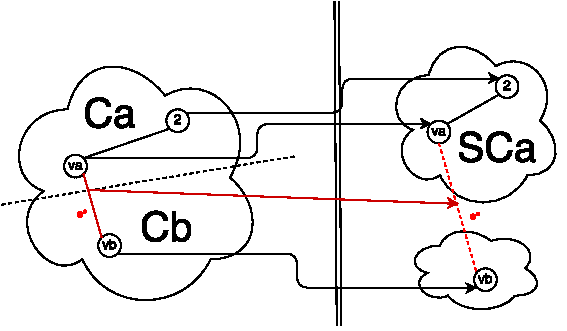
\includegraphics[width=1.4\textwidth,angle=90]{diagrama_ej2.pdf}
   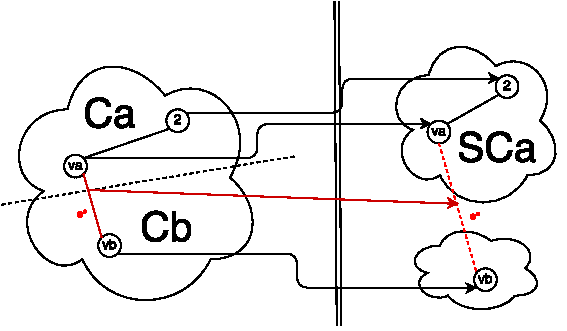
\includegraphics[width=1\textwidth]{diagrama_ej2.pdf}
   \caption{\textbf{Ejemplo gráfico del párrafo anterior}}
   \label{fig:ej2-1}
   \end{center}
\end{figure}

En el gráfico se puede apreciar el fenómeno expuesto en el párrafo anterior,
en donde a modo de ejemplo se están obviando los nodos que no son
imprescindibles a la demostración (se asume que adentro de las ``nubes'' hay
una cantidad indefinida de nodos, y se sabe que dentro de cada ``nube'' los
nodos son conexos).

\end{demostracion}

Dado que todas las soluciones de este problema tienen la misma cantidad de
nodos, ya que son subgrafos generadores de $K_n$, ya que la cantidad de nodos
contenidos en las \violet{$n-(i+1)$} componentes de \violet{$S^{*}$} suma $n$,
y teniendo en cuenta la proposición anterior, se deduce que las
\violet{$n-(i+1)$} componentes de \violet{$S^{*}$} están contenidas en
\redbf{a lo sumo $n-(i+1)$} componentes de \redbf{$S_{n-i}$} o, lo que es lo
mismo, que existe cierto conjunto de \red{\textbf{a lo sumo} $n-(i+1)$ componentes
de $S_{n-i}$ \emph{\textbf{cuyos nodos suman n}}}, y puesto que existen
\redbf{$n-i$} componentes en \redbf{$S_{n-i}$} eso significaría que entre
todas ellas sumarían como mínimo \redbf{$n + [ (n-i) - (n-(i+1)) ] = n+1$} nodos, lo cual es
\textbf{ABSURDO}.

\end{paragraph}

\end{document}